\documentclass{article}
\usepackage[margin=1in]{geometry}
\usepackage{amsmath,amsthm,amssymb}
\usepackage{bbm,enumerate,mathtools}
\usepackage{tikz,pgfplots}
\usepackage{chessboard}
\usepackage[hidelinks]{hyperref}
\usepackage{multicol} % Problem 35

\newenvironment{question}{\begin{trivlist}\item[\textbf{Question.}]}{\end{trivlist}}
\newenvironment{note}{\begin{trivlist}\item[\textbf{Note.}]}{\end{trivlist}}
\newenvironment{references}{\begin{trivlist}\item[\textbf{References.}]}{\end{trivlist}}
\newenvironment{related}{\begin{trivlist}\item[\textbf{Related.}]\end{trivlist}\begin{enumerate}}{\end{enumerate}}


\begin{document}
\rating{3}{3}
The prime ant looks along the number line starting at $2$. When she reaches a
composite number, she divides by its least prime factor, and adds that factor to
the previous term, and steps back.

\begin{figure}[!h]
  \centering
  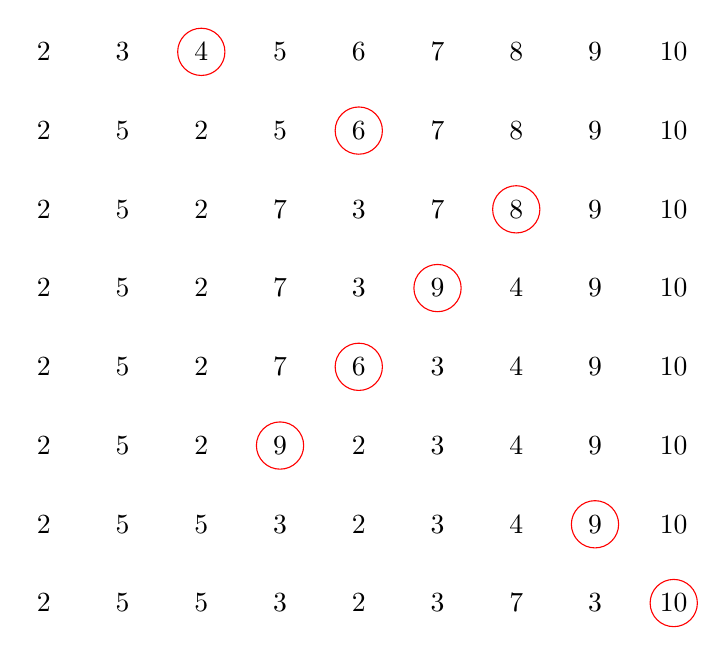
\begin{tikzpicture}
    \def\antsteps{
      0/{0/2,1/3,2/4,3/5,4/6,5/7,6/8,7/9,8/10}/2,
      1/{0/2,1/5,2/2,3/5,4/6,5/7,6/8,7/9,8/10}/4,
      2/{0/2,1/5,2/2,3/7,4/3,5/7,6/8,7/9,8/10}/6,
      3/{0/2,1/5,2/2,3/7,4/3,5/9,6/4,7/9,8/10}/5,
      4/{0/2,1/5,2/2,3/7,4/6,5/3,6/4,7/9,8/10}/4,
      5/{0/2,1/5,2/2,3/9,4/2,5/3,6/4,7/9,8/10}/3,
      6/{0/2,1/5,2/5,3/3,4/2,5/3,6/4,7/9,8/10}/7,
      7/{0/2,1/5,2/5,3/3,4/2,5/3,6/7,7/3,8/10}/8
    }

    \foreach \vertical/\ary/\circleposition in \antsteps {
      \draw[red] (\circleposition, -\vertical) circle (0.3cm);
      \foreach \horizontal/\nodename in \ary {
        \node at (\horizontal, -\vertical) {\nodename};
      }
    }
  \end{tikzpicture}
  \caption{An illustration of the prime ant's positions after the first 7 steps.}
\end{figure}

\begin{question}
  Does the ant eventually stay to the right of any fixed position?
\end{question}
\begin{related}
  \item Are there any positions that stay permanently greater than $7$? Than $11$?
  \item Does sequence of numbers converge in the long run? If so, what to?
    $(2, 5, 5, 3, 2, \hdots)$
  \item Let $S$ be a subset of $\mathbb{N}$ and let
    $f: S\times S^{c} \rightarrow \mathbb{N}^2$.
    For what ``interesting'' sets $S$ and functions $f$ can we answer the above
    questions?\\
    (In the example $S$ is the prime numbers and $f$ maps
    $(p, c) \mapsto (p + \operatorname{lpf}(c), \operatorname{gpf}(c))$.)
\end{related}
\begin{references}
  \item \url{https://codegolf.stackexchange.com/q/144695/53884}
  \item \url{https://math.stackexchange.com/q/2487116/121988}
  \item \url{https://oeis.org/A293689}
\end{references}
\end{document}
